\noindent This is the last topic that we need to complete our description of the standard model of elementary particle interactions. \textit{Spontaneous symmetry breaking} (SSB) is an observed behavior within field theories, and we will begin with some examples of classical SSB.

\subsubsection*{Particle in a double well example}

\noindent Consider a classical particle confined to a double-well potential with Hamiltonian

\begin{equation}
H = \frac{p^2}{2m} + V(x).
\end{equation}

\noindent This system posses $\mathbb{Z}_2$ symmetry in its solutions, since $x \rightarrow -x$ is a symmetry operation. Note that the particle in this potential at $x=0$ must choose a positive or negative local minimum, meaning that the ground state is degenerate and breaks the $\mathbb{Z}_2$ symmetry. \\

\begin{figure}[H]
	\centering
	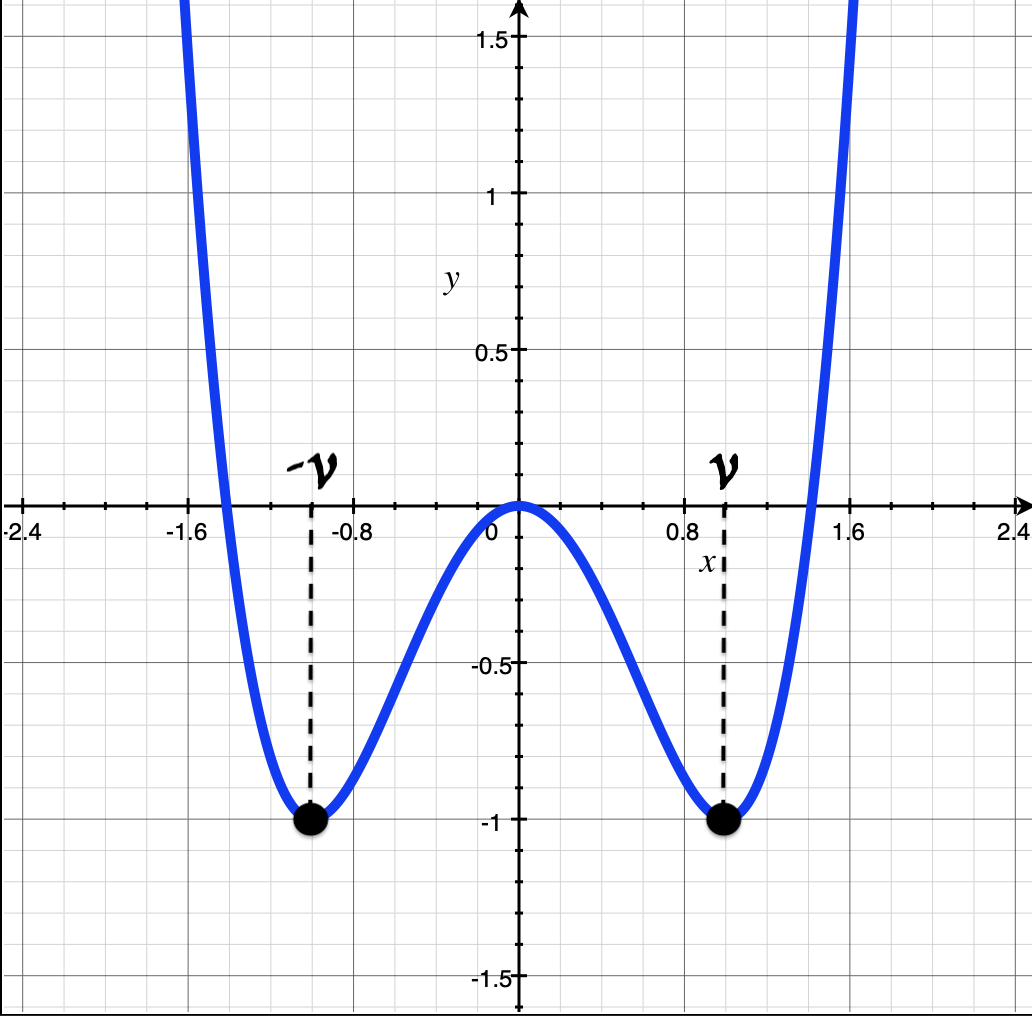
\includegraphics[width=3in]{images/mexhat2d.png}
	\caption*{Potential exhibiting $\mathbb{Z}_2$ symmetry.}
\end{figure}

\noindent The quantum analog of this classical theory does not exhibit SSB, since the ground state wavefunction is symmetric, but the first excited state is antisymmetric.

\begin{figure}[H]
	\centering
	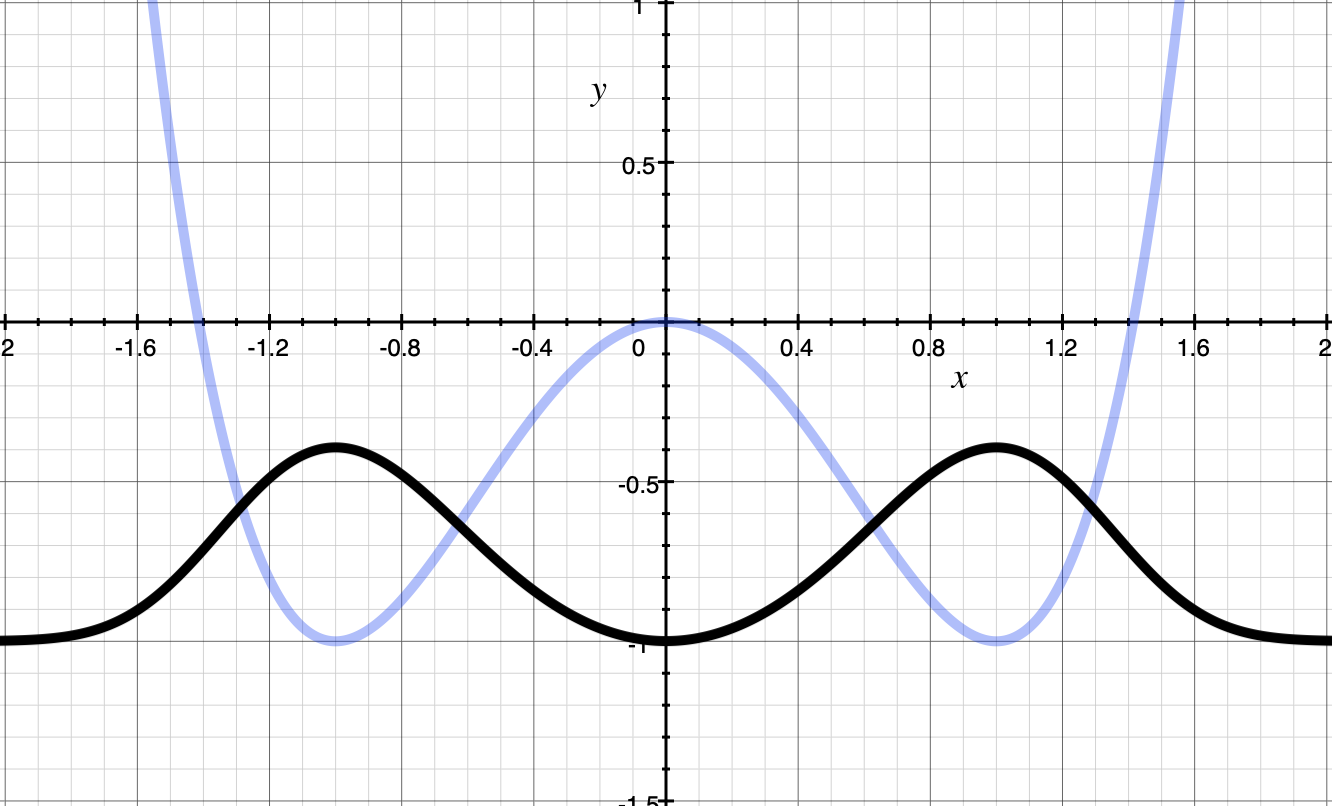
\includegraphics[width=2in]{images/mexhat2d_ground.png}
	\caption*{Symmetric ground state wavefunction.}
\end{figure}

\begin{figure}[H]
	\centering
	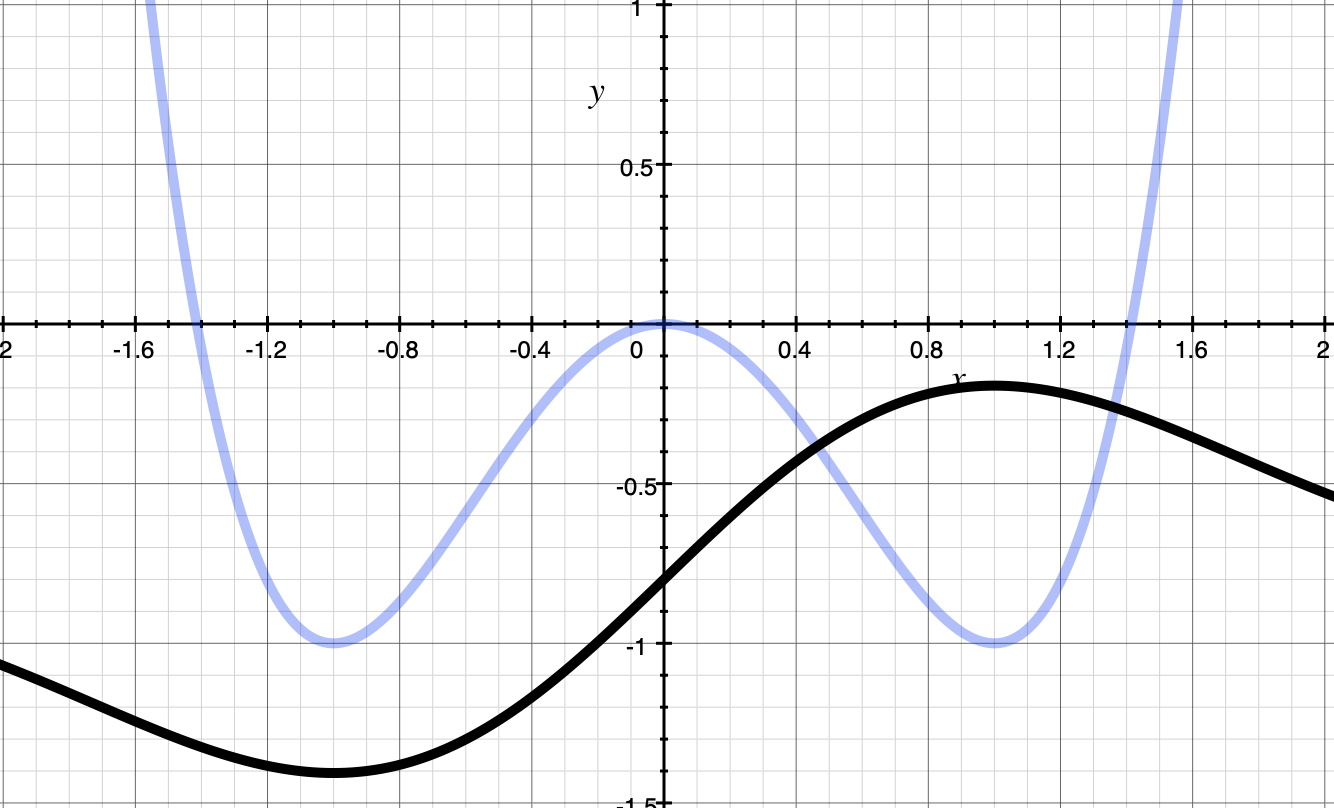
\includegraphics[width=2in]{images/mexhat2d_first.png}
	\caption*{Antisymmetric first excited state wavefunction.}
\end{figure}

\subsubsection*{Ising model (statistical physics) example}

\noindent The Ising model is a model of ferromagnetic materials, where spins can point up or down, corresponding to a spin value $s_j =  \pm 1$, with a Hamiltonian containing the pairwise summation

\begin{equation}
H = -\sum_{\langle jk \rangle} s_j s_k.
\end{equation}

\noindent This theory contains two ground states: all spins pointing up or all pointing down, and possesses $\mathbb{Z}_2$ symmetry by the operation $s_j \rightarrow -s_j$. \\

\noindent Depending on the temperature, the thermal state of this system can be in one of two regimes: critical or non-critical. Consider the Gibbs, or mixed, state density operator describing the system at any temperature

\begin{equation}
\rho = \frac{e^{-\beta H}}{Z}
\end{equation}

\noindent Where $Z$ is the partition function and $\beta = \frac{1}{k_B T}$ is the temperature factor. Note that the Gibbs state is all $\mathbb{Z}_2$ symmetric, meaning that it does break any symmetries. Now there exists a critical temperature $\beta_{c}$, below which the system becomes ordered due to small external magnetic fluctuations and symmetry is broken. Above the critical temperature, the system is disordered with random thermal fluctuations. As $\beta \rightarrow \infty$,

\begin{equation}
\rho = \left(\frac{1}{2} - \epsilon\right) (\text{all up states}) + \left(\frac{1}{2} - \epsilon \right)(\text{all down states}).
\end{equation}

\subsubsection*{Classical field theory example}

\noindent Consider the Lagrangian density, much like the $\phi^4$ interacting theory we've encountered, but the ``mass'' term is made negative and $m \rightarrow \mu$

\begin{equation}
\mathcal{L} = \frac{1}{2} (\partial_\mu \phi)(\partial^\mu \phi) + \frac{1}{2} \mu^2 \phi^2 - \frac{\lambda}{4!} \phi^4.
\end{equation}

\noindent Note that measurable quantities are usually functions of the parameters, making this a perfectly fine theory. We then have the Hamiltonian

\begin{equation}
H = \int d^3 x \, \left( \frac{1}{2} \pi^2 + \frac{1}{2} (\nabla \phi)^2 - \frac{1}{2} \mu^2 \phi^2 + \frac{\lambda}{4!} \phi^4 \right).
\end{equation}

\noindent To uncover the $\mathbb{Z}_2$ symmetry of this theory, minimize the Hamiltonian with respect to the field $\phi$, making all derivatives of $\phi$ equal to zero, and calculate the configuration with the smallest energy. The extremum condition for the remaining potential energy terms

\begin{equation}
\frac{\partial V(\phi)}{\partial \phi} = -\mu^2 \phi + \frac{\lambda}{6} \phi^3 = 0
\end{equation}

\noindent Yields three configurations that extremize the energy of the system. Namely, for $\phi = 0$ and $\phi = \pm \sqrt{\frac{6 \mu^2}{\lambda}}$. The quantum analog of this theory also exhibits SSB.

\subsubsection*{Quantum field theory example: transverse Ising model}

\noindent Consider the quantum theory of a 1D lattice of spins, which also exhibits $\mathbb{Z}_2$ symmetry, with the Hamiltonian

\begin{equation}
\hat{H} = - \sum_{j} \sigma_j^x \sigma_{j+1}^x + h \sum_j \sigma_j^z
\end{equation}

\noindent Where the first term is the neighboring interaction and the second term is the magnetic interaction with $h$ as the magnetic field strength, and the Pauli spin matrices

\begin{equation}
\sigma^x = \left( \begin{array}{cc} 0 & 1 \\ 1 & 0 \end{array} \right) \text{ and } \sigma^z = \left( \begin{array}{cc} 1 & 0 \\ 0 & -1 \end{array} \right).
\end{equation}

\noindent The Hamiltonian exhibits $\mathbb{Z}_2$ symmetry, since 

\begin{equation}
[\Phi,\hat{H}] = 0 \text{ for } \Phi = \dots \sigma_j^z \sigma_{j+1}^z \dots.
\end{equation}

\noindent The basis for the $h=0$ ground state can be written as

\begin{align}
\ket{\Omega_+} &\equiv \ket{+} \otimes \ket{+} \otimes \dots \otimes \ket{+} \\
\ket{\Omega_-} &\equiv \ket{-} \otimes \ket{-} \otimes \dots \ket{-}
\end{align}

\noindent Where the individual spin states are

\begin{equation}
\ket{+} = \frac{1}{\sqrt{2}} \left( \ket{0} + \ket{1} \right) \text{ and } \ket{-} = \frac{1}{\sqrt{2}} \left( \ket{0} - \ket{1} \right).
\end{equation}

\noindent The $h=0$ ground state eigenspace is twofold degenerate with the above basis. A good, non-degenerate ground state, for example, could be $\frac{1}{\sqrt{2}} ( \ket{\Omega_+} \pm \ket{\Omega_-} )$, but these states are never seen in experiment, since decoherence destroys any superpositions of states. Neither state by itself exhibits the symmetry, but one state must be chosen by measurement. The only information we have about the two states' relationship is $\Phi \ket{\Omega_+} = \ket{\Omega_-}$.

\subsubsection*{Continuous SSB Example: Linear $\sigma$-model}

\noindent Consider the Lagrangian density for an effective model of pions that exhibits SSB of a continuous symmetry

\begin{equation}
\mathcal{L} = \frac{1}{2}(\partial_\mu \phi^j )^2 + \frac{1}{2} \mu^2 (\phi^j)^2 - \frac{\lambda}{4!} (\phi^j)^4
\end{equation}

\noindent Where $(\phi^j)^2 = \sum_{j=1}^N \phi^j \phi^j$. The dynamics of the $N$ independent (Klein-Gordon) scalar field are invariant under orthogonal rotations $O \in O(N)$, a continuous group of symmetries, such that

\begin{equation}
O: \,\, \phi^j \rightarrow [O]^j_k \phi^k.
\end{equation}

\noindent What is the lowest energy configuration? Minimize the potential energy $V(\phi^j) = -\frac{1}{2} \mu^2 (\phi^j)^2 + \frac{\lambda}{4!} (\phi^j)^4$ with respect to $\phi^j$, showing that the minimum occurs for any constant configuration of the fields that satisfies the equation (\textbf{Exercise})

\begin{equation}
(\phi_0^j)^2 = \frac{\mu^2}{\lambda}. 
\end{equation}

\noindent There is more than one energy configuration that leads to this solution, including superpositions of the following vectors

\begin{equation}
\begin{pmatrix} \frac{\mu}{\sqrt{\lambda}} \\ 0 \\ 0 \\ \dots \\ 0 \end{pmatrix}, \begin{pmatrix} 0 \\\frac{\mu}{\sqrt{\lambda}} \\ 0 \\ \dots \\ 0 \end{pmatrix}, \dots .
\end{equation}

\noindent In the case of $N=2$, the potential energy minima form the ``wine bottle'' or ``mexican hat'' potential. The minimum energy configurations are points on this potential and form circles around the indent of the ``bottom of the bottle''. In other words, any configuration that lands on the circle is a minimum energy configuration.

\begin{figure}[H]
	\centering
	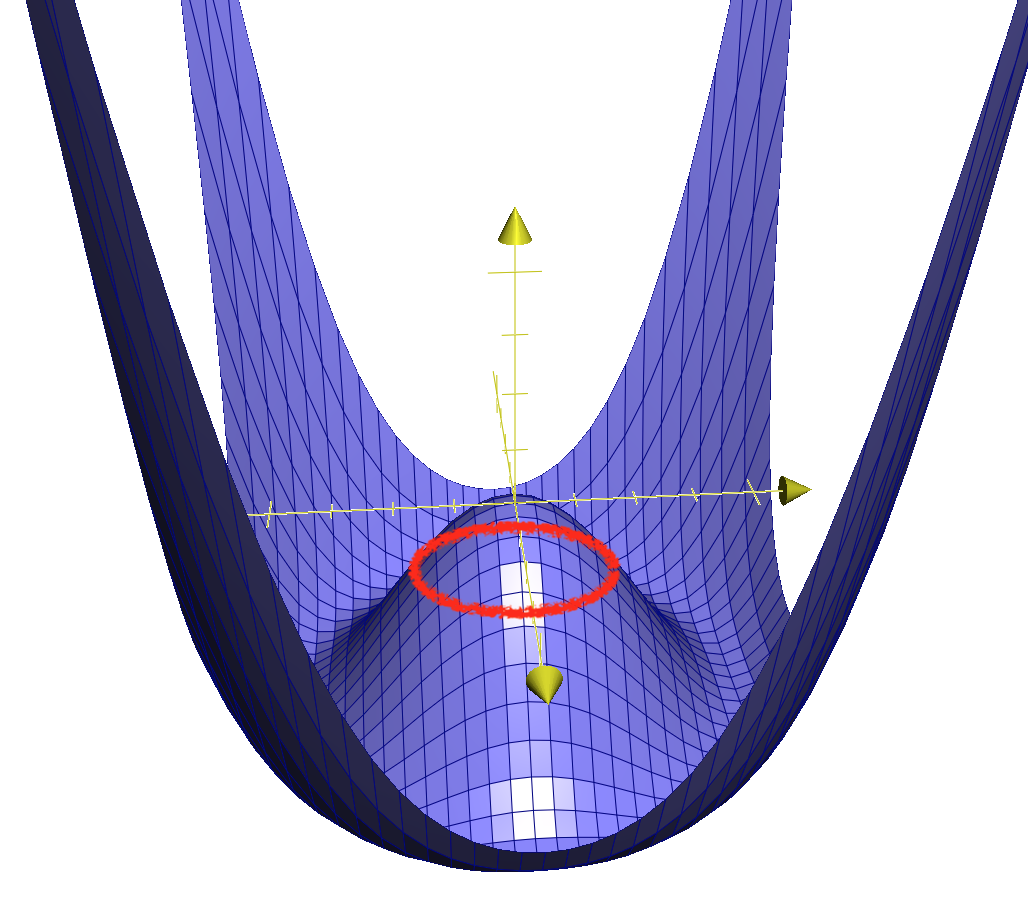
\includegraphics[width=3in]{images/mexhat3d.png}
	\caption*{Mexican hat potential of the linear sigma model.}
\end{figure}

\subsubsection*{Low Energy Dynamics for SSB}

\noindent To study the dynamics as we start to depart from the minimal energy configurations, the ground state, consider the $\mathbb{Z}_2$-symmetry case. Effectively, the low energy dynamics for a classical $\mathbb{Z}_2$-symmetric system are that of a harmonic oscillator with an effective mass, a restoring force. \\

\begin{figure}[H]
	\centering
	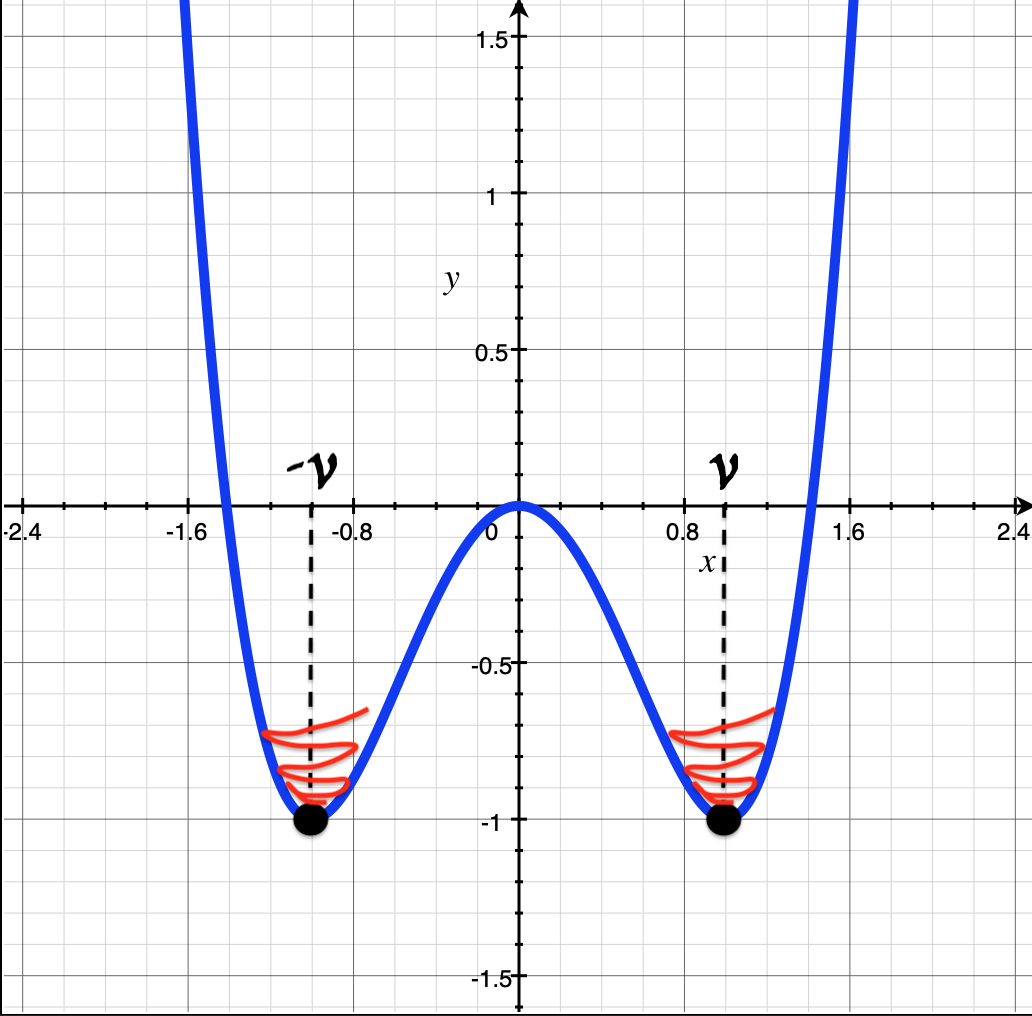
\includegraphics[width=2in]{images/mexhat2d_smalldev.png}
	\caption*{Small fluctuations in the energy behave much like the harmonic oscillator.}
\end{figure}

\noindent In the continuous case, we choose coordinates by rotating such that

\begin{equation}
\phi_0^j = \begin{pmatrix} 0 \\ 0 \\ \dots \\ \nu \end{pmatrix} = \begin{pmatrix} 0 \\ 0 \\ \dots \\ \frac{\mu}{\sqrt{\lambda}} \end{pmatrix}
\end{equation}

\noindent And see how this behaves with small energy fluctuations. Define \textit{shifted fields} in terms of some new coordinates where the vector of fields $\underline{\phi}$ is now defined as

\begin{equation}
\underline{\phi} (x) \equiv ( \pi^k (x), \nu + \sigma (x) ) \text{, where } k = 1, \dots , N-1.
\end{equation}

\noindent Note that $\pi$ is not the conjugate momentum density, but a new classical field, which will be, hence the notation, the pion, and $k$ denotes the vector index.

\noindent Rewrite $\mathcal{L}$ in terms of the shifted fields (\textbf{Exercise})

\begin{align}
\mathcal{L} = &\frac{1}{2} (\partial_\mu \pi^k)^2 + \frac{1}{2} (\partial_\mu \sigma)^2 \\
& - \frac{1}{2} \left( 2 \mu^2 \sigma^2 - \sqrt{\lambda} \mu \sigma^3 - \sqrt{\lambda} \mu (\pi^k)^2 \sigma - \frac{\lambda}{4} \sigma^4 - \frac{\lambda}{2} (\pi^k)^2 \sigma^2 - \frac{\lambda}{4} (\pi^k)^4 \right).
\end{align}

\noindent There are $N-1$ massless $\pi^k$ fields and one massive $\sigma$ field. The second and third terms in $\mathcal{L}$ correspond to an effective massive Klein-Gordon scalar field. The $N-1$ $\pi^k$ fields are effectively massless, as all of the other terms above contain $\lambda$ and are interaction terms. \\

\noindent It costs energy to move transverse in the potential, perpendicular to the circle of minima, corresponding to the effective mass of the $\sigma$ field. To move tangentially to the manifold of minima, the circle, it costs no energy, corresponding to the massless $\pi$ fields. \\

\subsubsection*{Goldstone's Theorem}

\noindent In the $O(N)$ linear $\sigma$-model there are ${N \choose 2}$ independent continuous symmetries, the dimension of the rotation group $O(N)$. After SSB, there are ${N-1 \choose 2}$ remaining symmetries, the dimension of $O(N-1)$, corresponding to rotations of the $\pi^k$ fields. The number of broken symmetries is equal to ${N \choose 2} - {N-1 \choose 2} = (N-1)$, which is also the number of massless fields. In other words, each broken symmetry causes a massless excitation: the \textit{Goldstone modes} or \textit{Goldstone bosons}. \\

\noindent \textbf{Therorem:} For every broken symmetry, there is a corresponding massless bosonic particle. \\

\noindent \textbf{Proof:} \\

\noindent Consider a classical field theory with fields $\phi^a (x)$, $a = 1, 2, \dots$, and the general Lagrangian density $\mathcal{L} = (\text{derivatives}) - V(\phi^a)$. \\

\noindent Let $\phi_0^a$ be a constant (in an extrema) field that minimizes the potential such that

\begin{equation}
\frac{\partial V(\phi^a)}{\partial \phi^a} \Big{|}_{\phi^a = \phi_0^a} = 0.
\end{equation}

\noindent Then expand the potential, a function of the vector of fields $\phi^a_0 \equiv \underline{\phi}_0$, near the minima

\begin{equation}
V(\phi^a) = V(\phi^a_0) + \frac{1}{2} (\phi^a - \phi_0^a) (\phi^b - \phi_0^b) \left( \frac{\partial^2 V}{\partial \phi^a \partial \phi^b} \right) \Big{|}_{\phi=\phi_0}.
\end{equation}

\noindent Call the Hessian matrix $[m^2]_{ab}$, which is symmetric and real and the eigenvalues give the masses of the effective fields. \\

\noindent With an orthogonal rotation, we can diagonalize a symmetric, real matrix $m^2 \rightarrow O^T D O$. Redefine the fields $\pi^a = [O]^a_b \phi^b$, and rewrite the Lagrangian density

\begin{equation}
\mathcal{L} (\pi^a) = (\text{derivatives}) - \sum_a D_a^2 (\pi^a)^2
\end{equation}

\noindent Where the eigenvalues correspond to the masses of the $\pi$ particles, and we must now show that there are eigenvalues equal to zero. In other words, every continuous symmetry leads to an eigenvalue equal to zero. \\

\noindent A general, global, continuous symmetry of the fields has the form

\begin{equation}
\phi^a \rightarrow \phi^a + \alpha \Delta^a (\phi)
\end{equation}

\noindent Where $\alpha$ is infinitesimal and $\Delta^a$ is a shift function of the fields. This is a symmetry of the potential, since it causes the derivatives to vanish such that

\begin{equation}
V(\phi^a) = V(\phi^a + \alpha \Delta^a (\phi)).
\end{equation}

\noindent This implies, by expanding and equating first order terms, the directional derivative of the potential is zero

\begin{equation}
\Delta^a (\phi) \frac{\partial}{\partial \phi^a} V(\phi) = 0.
\end{equation}

\noindent Differentiate this with respect to $\phi^b$ to get

\begin{equation}
\frac{\partial \Delta^a (\phi)}{\partial \phi^b} \frac{\partial V(\phi)}{\partial \phi^a} + \Delta^a (\phi) \frac{\partial^2 V}{\partial \phi^a \partial \phi^b} = 0.
\end{equation}

\noindent Evaluate at $\phi^a = \phi_0^a$ to get

\begin{equation}
\sum_a \Delta^a (\phi_0^a) [m^2]_{ab} = 0
\end{equation}

\noindent Where $\sum_a \Delta^a (\phi_0^a) = \Delta^T$ is the zero eigenvector, where the $\Delta^a (\phi^a_0)$ are linearly independent for each continuous symmetry, which follows by definition of the general, global, continuous symmetry imposed above.